% TEMPLATE for Usenix papers originally for producing IEEE-format articles
% written by Matthew Ward, CS Department, Worcester Polytechnic Institute.
% adapted by David Beazley for his paper in Proceedings, Tcl 96
% turned into a smartass generic template by De Clarke

\documentclass[twocolumn,10pt]{article}
\usepackage[margin=1in]{geometry}
\usepackage{graphicx,subcaption,hyperref}

\title{6.829 Final Project: A comparison of bit-rate selection algorithms}
\author{Colleen Josephson \\ \texttt{cjoseph@mit.edu}
  \and Pavel Panchekha \\ \texttt{pavpan@mit.edu}}
\date{May 2013}

\begin{document}
\maketitle

\begin{abstract}
We compare the performance SampleRate and Minstrel, two popular
bit-rate selection algorithms that have widespread real-world usage.
We use a trace-based approach to avoid kernel programming and consider
Python implementations of both SampleRate and Minstrel.  We test both
algorithms in multiple real-world scenarios, including scenarios with
mobile clients and noisy environments, to highlight differences
between the two algorithms.  We also introduce improvements to the
Minstrel algorithm that allow for significant gains in throughput.
\end{abstract}

\section{Introduction}

One of the key ways that wireless networks differ from wired links is
that wireless networks have varying link rates.  Link conditions vary
with time due to interference from other devices, changing network
geometry, and mobile clients.  An optimal rate at one time may be
different from the optimal rate just 30 seconds earlier.  A good
bit-rate selection algorithm has to detect and adapt to these
conditions.  If the chosen bit-rate is too slow, then the throughput
will be unnecessarily low; if the rate is too high, failures will be
very frequent and throughput will again suffer.

There are three main classes of bit-rate adaptation protocols:
frame-based, SNR-based, and cross-layer protocols.  Frame-based
protocols measure the fraction of successfully received packets.  SNR
protocols make decisions based on the estimated Signal to Noise ratio.
Cross-layer protocols use SoftPHY data from the physical layer.  The
most commonly implemented protocols on today's networks are frame
based, because SNR protocols perform poorly~\cite{samplerate}, and
cross-layer protocols cannot be deployed on current networks as they
violate the network layering abstraction.

The two most popular frame-based protocols are SampleRate and
Minstrel.  Both were implemented in the MadWifi drivers for Linux
wireless, and today Minstrel is the default bit-rate selection
algorithm for all wireless drivers on Linux.  Our research used a
trace-based approach to analyze the performance of these two
algorithms.  We also created a modified version of Minstrel that
provides significant throughput gains over the vanilla Minstrel
implementation.

This paper will provide a general overview of SampleRate and Minstrel.
We then discuss our testing methodology.  We compare the performance
of the two algorithms, and then discuss modifications we made to
Minstrel and compare it's performance to the current kernel
implementation.


\section{SampleRate}

SampleRate, first introduced in \cite{samplerate}, is a bit rate
selection algorithm which maintains estimates of average transmission
time for each potential bit rate.To keep these estimates up to date,
SampleRate periodically sends a packet at a randomly-selected bit
rate, and uses the success or failure of this packet to update the
average transmission time of that bit-rate.  SampleRate also abandons
a bit rate after four successive failures at that rate.  All
information about packets is maintained with a 10-second sliding window.

SampleRate has three main functions: \texttt{ApplyRate()}, which
returns a the bit-rate to send a packet at,
\texttt{ProcessFeedback()}, which updates the statistics for a
bit-rate after an attempted packet send, and
\texttt{RemoveStaleResults()}, which removes the effect of packets
older than 10 seconds.

\section{Minstrel}

Minstrel, developed specifically for the Linux kernel, attempts to
improve upon SampleRate to make it better suited for noisy or
dynamic environments.  Unlike SampleRate, Minstrel tracks raw
probabilities of successful transmission for each bit rate, computed
based on an exponentially-weighted moving average of 100ms windows.

Minstrel makes use the multi-rate retry chain (MRR), an array of bit rates
and number of attempts to make at each bit rate, that tells the card
which rates to try before reporting a failure.  The retry chain makes
failures extremely unlikely and allows Minstrel to choose fallback
rates when a packet does not succeed.  Minstrel sets the MRR to first
try the rate with the highest throughput, then the next-highest
throughput, then greatest probability of success, and finally attempts
to send a packet at the lowest, base rate.  In essence, Minstrel tells
the card to send at the highest throughput rates but to fall back to
reliable rates upon failure.

To keep an accurate estimate of throughput and probability for each
rate, Minstrel sends sample frames ten percent of the time.  However,
Minstrel tries to avoid sampling at a rate slower than the current
best rate, if the current best rate is still successfully
transmitting.  If the randomly chosen rate has a higher lossless
throughput than the current optimal rate, the MRR first lists the
sample rate, then the highest-throughput rate, then the
best-probability rate, and finally the base rate.  On the other hand,
if the random rate is slower than the optimal rate, the sample rate is
placed lower in the retry chain: first, the best throughput rate is
tried, and only if it fails does the sample rate then get attempted
(followed, as usual, by the best probability rate and the base rate).
This ensures that Minstrel never samples rates worse than the current
optimal rate unless the optimal rate experiences a failure.  See
Table~\ref{table:mrr} for an overview of the retry chains used in
Minstrel.

Minstrel implementation is based on SampleRate, so it also has
\texttt{ApplyRate()} and \texttt{ProcessFeedback()} methods, as well
as a \texttt{UpdateStats()} method that runs every 100ms.
\texttt{UpdateStats()} is home to some of the key differences between
Minstrel and SampleRate.  Instead of making decisions based on the
average transmission time, Minstrel uses throughput, computed with $$T
= \frac{p}{tx\_time}$$ where $T$ is the throughput of some rate $r$,
$p$ is the probability of successfully transmitting at $r$, and
$tx\_time$ is the computed lossless transmission time at rate $r$.

The probability $p$ of a successful transmission is calculated from
statistics collected by the \texttt{ProcessFeedback()} method, and is
done using an exponential weighted moving average, or EWMA.  The EWMA
creates a weighted average that weighs recent data more heavily than
old data, with the weighting for old data decreasing exponentially.
An EWMA ensures that a sudden degradation in link quality will create
a rapid response in the probabilities, making the EWMA-using Minstrel
perform better in dynamic environments.  Minstrel will waste less time
sending packets at a rate that no longer works, as compared to a
simple sliding-window probability calculation.

\begin{table*}[htb]
  \centering
    \begin{tabular}[htb]{l|l|l|l}
    \textbf{Try} & \textbf{Normal} &
    \textbf{Random (slower than best)} &
    \textbf{Random (faster than best)} \\ \hline
    1 & Best throughput      & Best throughput     & Random              \\
    2 & Next best throughput & Random              & Best throughput     \\
    3 & Highest probability  & Highest probability & Highest probability \\
    4 & Lowest rate          & Lowest rate         & Lowest rate         \\
    \end{tabular}
    \caption{Multi-rate retry chains for Minstrel}
\label{table:mrr}
\end{table*}

\section{Methodology}

We collected traces about the success rates of each bit rate through a
modified Linux wireless driver; Minstrel and SampleRate were then
re-implemented in Python and replayed on this collected data.

\subsection{Motivation}

Our initial plan was to use the algorithms as implemented in the
MadWifi drivers for the Atheros chip.  However, MadWifi is deprecated,
and only runs on now-ancient network cards.  In addition to the
unavailability of compatible hardware, MadWifi would not be an
accurate reflection of contemporary users.  Both ath5k and
\texttt{ath9k}, which were created to replace MadWifi, did not port
the old bit-rate selection system from MadWifi and instead opted to
use the Linux kernel's rate selection framework, which only implements
Minstrel.  Porting SampleRate over to the new drivers would not have
been trivial, as there are vast differences in the assumed interfaces.

At this point, we decided to take a different approach and use an
approach similar to that used in Sprout~\cite{sprout}.  We modified
the \texttt{ath9k} driver to try bit rates uniformly and report packet
successes and failures, then analyze this data in user-space with
re-implementations of SampleRate and Minstrel.  Not only did this
lessen the re-implementation cost (since the algorithms were
re-implemented in user-space in Python, not in kernel-mode in C), but
it also provided reproducibility and allowed us to investigate
modifications to SampleRate and to Minstrel.

\subsection{Trace Collection}

Traces were collected from an \texttt{ath9k} driver modified to sample
bit-rates uniformly (forgoing the usual bit rate selection algorithm)
and to report successes and failure from each packet.  Each bit-rate
was sampled uniformly in time -- thus, more packets were sent at
higher bit-rates, since those bit-rates otherwise deliver packets
faster.  For each packet sent, the time to send was recorded, and the
bit rate for the next packet was chosen to be the bit-rate that had
the smallest total transmissions time.  This guarantees approximately
uniform selection of bit-rates.  The wireless card used was an
Qualcomm Atheros \texttt{AR9285} Wireless Network Adapter.

Traces were collected at an unused access point in a basement of MIT.
Before initiating trace collection, the wireless card was put in
monitor mode for a minute to check that no other users were connected
to the access point.  None were, guaranteeing that traces would not
include delays from carrier sensing or run into problems due to
congestion at the access point.  Traffic was simulated by sending 1500
byte packets to the access point's IP address.  Packets were sent over
UDP to avoid the TCP congestion window and retry loop; since no users
were using the access point, there was no real risk of deteriorating
service for other users.  Figure~\ref{figure:1} shows a floor plan of
the access point and basement.

Eighteen total traces were collected, grouped into a number of
scenarios.  Each trace was 30 seconds to a minute long, and each
scenario was repeated twice.  One scenario placed the wireless card
with line of sight to the access point, two meters from it.  Another
created solid body interference by having one of the authors stand
between the wireless device and the access point.  One placed the
device around a corner from the access point, creating some potential
for multi-path interference and fading.  In one scenario, we moved the
wireless device throughout the trace, pacing back and forth in a 10
meter line in front of the access point.  Finally, one five-minute
trace was taken, which mixed the above scenarios, first moving around
a corner, then standing still, then moving to line-of-sight with the
access point.  A few shorter (3 to 15 second long) traces were
collected to investigate the startup behavior of bit-rate selection.

\begin{figure}[htbp]
  \centering
  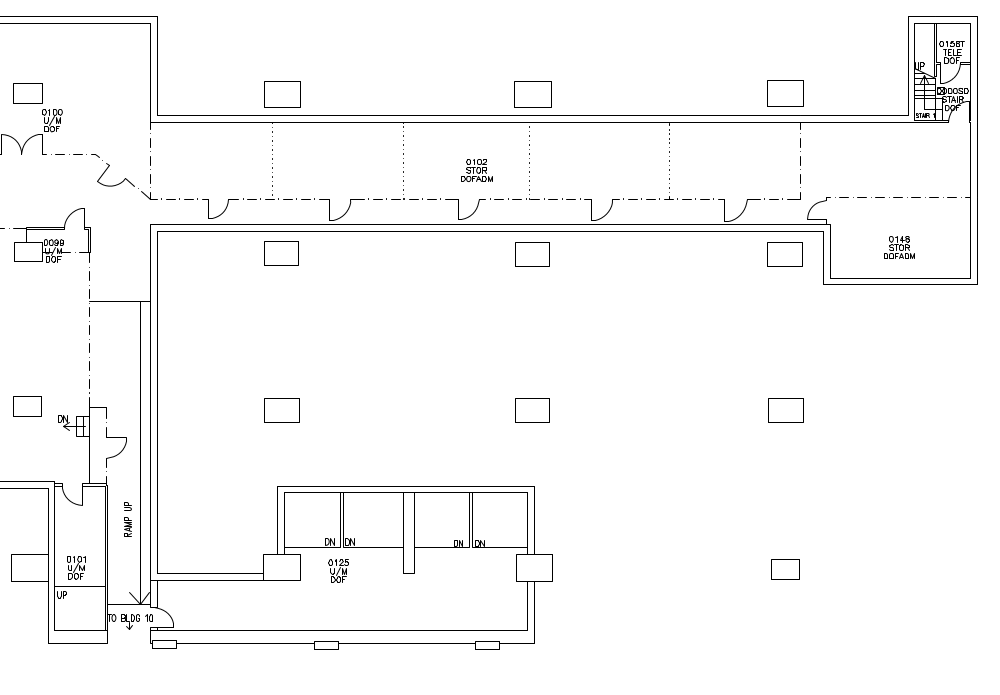
\includegraphics[width=\linewidth]{bsmt13floorplan.png}
  \caption{We collected most traces at a remote access point in the basement of Building 13 at MIT.}
\label{figure:1}
\end{figure}


\subsection{Testing framework}

Once collected, traces were fed to a bit rate selection simulator to
analyze the performance of Minstrel and SampleRate.  Both algorithms
were represented by two functions: \texttt{ApplyRate}, which returned
a multi-rate retry chain of rates to attempt transmission at, and
\texttt{ProcessFeedback}, which was passed the success or failure of
the transmission and how many attempts were made at each bit rate
(along with the current time and the total time to send the packet);
this parallels the interface used by the Linux kernel itself.  Helper
functions, like SampleRate's \texttt{RemoveStaleResults} function,
were instead called from one of \verb|apply_rate| or
\verb|process_feedback|.  For every packet transmission, the simulator
would call \texttt{ApplyRate}; compute the probability of success
based on packets sent in 10-millisecond window around the current
time; and from that determine the success or failure of the packet,
and the number of retries required.  The results of a test run are
thus non-deterministic; both algorithms tested are non-deterministic
anyway, so this is no handicap.  To improve re-implementation
fidelity, both implementations were meticulously checked by both
authors.

We implemented SampleRate as outlined in John Bicket's Master's
thesis~\cite{samplerate}.  This implementation is slightly different
from how it was implemented in the MadWifi kernel driver.  The primary
difference is that the kernel implementatiion uses a EWMA, while the
thesis implementation computes average transmission times based on a
10-second sliding window.  It would be worth looking at the
performance of EWMA-based SampleRate in the future.  Our
implementation, \texttt{samplerate.py} contains \texttt{ApplyRate()},
\texttt{ProcessFeedback()} and \texttt{RemoveStaleResults()}, as well
as a few helper functions and data structures for tracking rate
statistics.

We implemented Minstrel by porting the C code from the 3.3.8 version
of the Linux kernel into Python.  \texttt{minstrel.py} contains
\texttt{ApplyRate()}, \texttt{ProcessFeedback()} and
\texttt{UpdateStats()}, as well as a few helper functions and data
structures for tracking rate statistics.

\subsection{Experimental parameters}

There are a few parameters that can be adjusted in Minstrel and
SampleRate, but our implementation is consistent with what the
respective authors originally chose.

In SampleRate, the number of successive retries, the frequency of
probe packets, the window size, and the lossless $tx\_time$
estimations are all parameters that can be changed.  The SampleRate
thesis chose 4 successive retries, a probe frequency of every ten
packets, and a window size of ten seconds.  We used the same values in
our implementation.  Additionally, we use the same equation to
calculate $tx\_time$.

In Minstrel, the frequency of probe packets, the window size, and the
EWMA weighting are the adjustable parameters.  The 3.3.8 Linux kernel
uses a probe frequency of 10\%, a window size of 100ms, and a EWMA
weighting of 0.75.  We use the same values.  Additionally, Minstrel
also estimates $tx\_time$ using the \verb|ieee80211_frame_duration()|
method from the \texttt{util.c} file in \texttt{net/mac80211}.  We
implemented the same function in Python.


\section{Analysis} \label{sec:analysis}

Minstrel and SampleRate perform similarly, usually within 3 Mbps of
each other.  In especially noisy situations, such as when the client
is moving or when the client is around the corner from the access
point, Minstrel consistently outperforms SampleRate.
Figure~\ref{figure:3} shows the results of a single run of both
Minstrel and SampleRate over all the different types of traces we
collected.  This is consisten with the literature---the authors of
Minstrel noted that they focused on making Minstrel robust to poor
conditions~\cite{minstrel}, which means losing potential througput
gains in stable situations.  Conversely, John Bicket noted that
SampleRate performs better in stable situations than noisy or highly
varying conditions~\cite{samplerate}.  We were slightly surprised to
see how significantly SampleRate outperformed Minstrel in certain
situations, though, with throughput being up to $67\%$ higher.

\begin{figure*}[htbp]
  \centering
  \begin{subfigure}{.45\linewidth}
    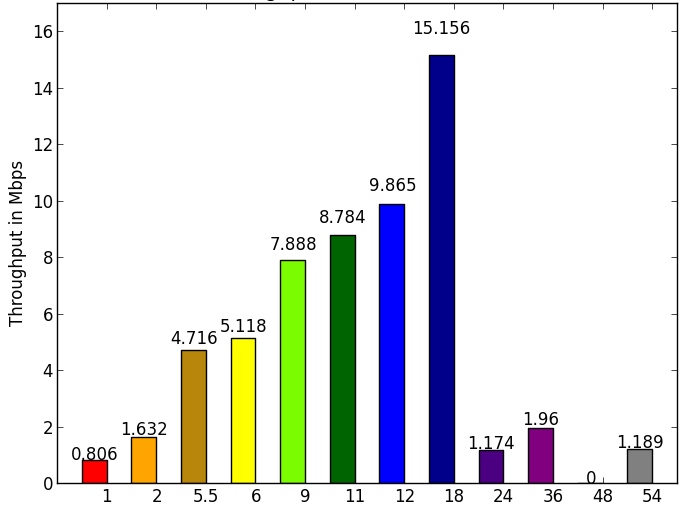
\includegraphics[width=\linewidth]{constant.png}
    \caption{Throughput of using a constant 802.11b/g bit-rate in
      clear line-of-sight from the access point.}
    \label{figure:2}
  \end{subfigure}\hfill
  \begin{subfigure}{.45\linewidth}
    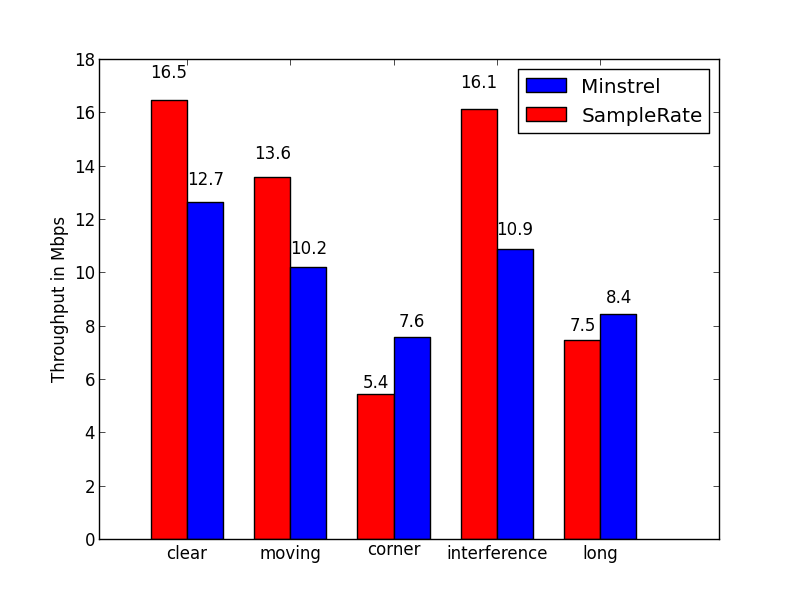
\includegraphics[width=\linewidth]{MinVSSam1.png}
    \caption{Throughput of Minstrel and SampleRate in various
      scenarios.}
    \label{figure:3}
  \end{subfigure}
  \caption{Comparing Minstrel and Samplerate}
\end{figure*}

In Figure~\ref{figure:2} we show the performance of constant bit-rates
on the \texttt{clear\_1.dat} trace, which is a 35 second trace in
clear view of the access point.  The optimal rate here was 18 Mbps,
which achieved an average throughput of about 15 Mbps.  The next
highest bit-rate, 24 Mbps, shows a large plummet in performance, down
to a throughput of 1.17 Mbps.  This steep drop is charateristic, and
is also talked about in the SampleRate thesis~\cite{samplerate}.  It
demonstrates just how important bit rate selection is---the optimal
bit rate has typically much higher throughput than the next-best rate,
but if the algorithm strays too high the results can be devastating.

Bit rate selection algorithms strive to have a throughput near or
greater than the optimal constant rate.  For this \verb|clear_1.dat|
trace, SampleRate clearly meets this goal, achieving an average
throughput more than 1 Mbps higher than the optimal constant rate.  In
noisier situations, though, Minstrel tends to be closer to the optimal
constant rate.

Bit rate selection algorithms naturally show variation between runs on
the same data because probe rates are chosen randomly.  The variations
were small, though.  On ten runs on the \texttt{clear\_1.dat} trace,
the average of Minstrel over 10 runs was 7.52 Mbps, with a maximum
variation of +/- 0.12 Mbps.  SampleRate was similarly stable, it
averaged 5.284 Mbps over 10 runs, with a maximum variation of about
+/- 0.3 Mbps.  The variation of results on other traces (except the
very short traces, where variance was naturally higher) was similar.

The histograms of which rates the algorithms decided to send at
provided some useful insight into their behavior.  Table~\ref{table:2}
is a histogram of a 35 second corner trace.  In this situation
Minstrel outperforms SampleRate.  The constant rate throughputs
demonstrate that 11, 12 and 18 Mbps were the optimal rates to send at,
and that no packets were sucessful at any higher rates.  SampleRate
does not use these rates except for probe packets, which happens once
every ten seconds.  Minstrel, since it does not terminate transmission
after four successive failures, spends a lot of time sending probe
packets at these high rates, which are never successful.  The only
reason low rates have fewer probe packets is because Minstrel
explicitly places them second in the retry chain, and because the main
rate usually succeeds.  Despite the fact that SampleRate spends less
time probing high rates, it is less successful.  This is because
Minstrel send the most packets at the three most successful bit-rates.
SampleRate, however, spends too much time sampling low bit rates.
Additionally, it spends a lot of time sending at 5.5 Mbps.  We suspect
that this might be because the equation SampleRate uses to estimate
average transmission time needs to be tweaked.
%   TODO: why does SampleRate spend time at 5.5 Mbps???

Our examination of the histograms showed us that Minstrel spends a lot
of time sampling at high rates.  In the specific case we examined, they
were all probe packets.  But sometimes Minstrel would choose 54Mbps as
the rate with the best throughput, which made little sense.  A closer
investigation revealed that Minstrel would sometimes get lucky with a
successful probe at 54Mbps.  The probability of success would be 1, so
then 54Mbps would be chosen as the rate with the best throughput.  This
is unfortunate, but the real harm comes in the next window: packets
would now be send at 54Mbps, and nearly all would fail.  However,
since these hundreds of failed packets weight equally with the single
successful probe packet, Minstrel still considers 54 Mbps the best
rate.  Thus the probability of success might drop from 1 to about 0.70,
which is still high enough for the throughput equation to rank 54 Mbps
highly.  Fundamentally, the problem is that the EWMA does not account
the second block having hundreds more packets than the first.  In the
next section we will talk about Minproved, an improved version of
Minstrel where we attempt to fix this problem.


\section{Improvements to Minstrel}

In Section~\ref{sec:analysis}, we noted that the EWMA used by Minstrel
causes problems when probe packets succeed.  A natural next step was
to modify Minstrel to avoid this problem, by weighing each 100ms block
of statistics in proportion to how many packets it contains.  To
preserve the exponential weighing of statistics, we chose to weigh
each 100ms block based on the number of packets sent, compared to the
those sent in the average block.  Parameters were chosen so that if
all blocks were of average size, our ``balanced'' EWMA would behave
identically to a normal EWMA.

To achieve, this weighing, we first recast the usual EWMA algorithm.
The usual algorithm computes $$p \gets \alpha p + (1 - \alpha)
\frac{n_i}{d_i}),$$ where $p$ is the EWMA probability, $\alpha$ is a
weight factor equal to $0.75$ in Minstrel, and $n_i$ and $d_i$ are the
number of successful and total packets in the 100ms window.  We next
write this as $$p \gets \frac{\beta p + \frac{n_i}{d_i}}{\beta + 1},$$
where $\beta = \alpha / (1 - \alpha)$.  We can now change the factor
in front of $n_i / d_i$ to account for the total number of packets
sent.  In our case, we chose to compute $$p \gets \frac{\beta p + w_i
  \frac{n_i}{d_i}}{\beta + w_i},$$ where the weight $w_i$ is $d_i / (d
/ b)$, with $d$ the total number of packets ever send and $b$ the
total number of 100ms windows ever seen.  Then $d / b$ is the average
number of packets per window and $d_i / (d / b)$ is the ratio between
the current window and the average window.  Note that if the current
window is of average size, this is exactly equal to the usual EWMA
result.  Finally, we can simplify the above equation to $$S p \gets
\frac{\beta \frac{d}{b} p + S n_i}{\beta \frac{d}{b} + d_i},$$ where
$S$ is any constant.  This equation is usable in fixed-precision
arithmetic, making it simple to implement in the Linux kernel (which
prefers to avoid floating point computations for portability reasons).
Because packets are high rates rarely succeed, the average window size
is a few packets; thus, the main qualitative difference between our
balanced EWMA and the original Minstrel EWMA is that non-probe packets
at probe bit-rates are weighed extraordinarily heavily, and this fact
allows us to avoid multiple failing 100ms windows.

We tested a modified Minstrel which used this more balanced EWMA
algorithm on the same traces as Minstrel and SampleRate, and found a
consistent improvement of approximately 1 Mbps over the normal
Minstrel algorithm.

We noted another curious fact about Minstrel: the kernel
implementation of Minstrel samples rates very frequently.  This is due
to a flag the kernel uses to track which probe bit-rates were actually
sampled.  In cases where the probe packets are at a lower bit-rate
than the current bit-rate, the probe packets might never be sent if
the current bit-rate succeeds.  However, the flagging seems to
misbehave in certain cases, causing the extremely aggressive probing
we see in some traces.  For example, in one of the traces where the
client was around a corner from the access point, Minstrel sent almost
half of its packets at probe frequencies.  We modified Minstrel to be
less aggressive with probe packets, decreasing the sampling frequency
to approximately 10\%.  This lead to more improvement, especially on
noisy traces such as the cases where the client was around a corner or
moving.

\begin{table*}[htb]
    \centering
    \begin{tabular}{l|l|l|l|l}

    \textbf{Rate in Mbps} & \textbf{SampleRate} &
    \textbf{Minstrel} & \textbf{Minproved} &
    \textbf{Constant Rate Throughput}\\ \hline

    1   & 631  & 39    & 29    & 0.639 Mbps \\
    2   & 863  & 82    & 20    & 1.425 Mbps \\
    5.5 & 4814 & 110   & 805   & 4.406 Mbps \\
    6   & 423  & 137   & 276   & 4.603 Mbps \\
    9   & 553  & 327   & 57    & 4.630 Mbps \\
    11  & 3326 & 4121  & 3356  & 9.627 Mbps \\
    12  & 4649 & 9515  & 14285 & 9.444 Mbps \\
    18  & 1154 & 13295 & 15795 & 8.458 Mbps \\
    24  & 16   & 6909  & 1918  & 0 Mbps \\
    36  & 16   & 6944  & 2030  & 0 Mbps \\
    48  & 16   & 6888  & 2009  & 0 Mbps \\
    54  & 16   & 7308  & 1953  & 0 Mbps \\ \hline

    \textbf{Avg. Throughput:} & \emph{5.42 Mbps}  & \emph{7.578 Mbps} & \emph{11.107 Mbps} \\
    \end{tabular}
    \caption{Histograms of the number of packets sent at each rate.
      The trace was \texttt{corner\_1.dat} and was recorded around the
      corner from the access point.  The best fixed rate for this
      trace was 11 Mbps, which achieved a throughput of 9.627 Mbps.
      Minproved achieves a higher throughput than the best fixed
      rate.}

    \label{table:2}
\end{table*}

\begin{figure}[htb]
  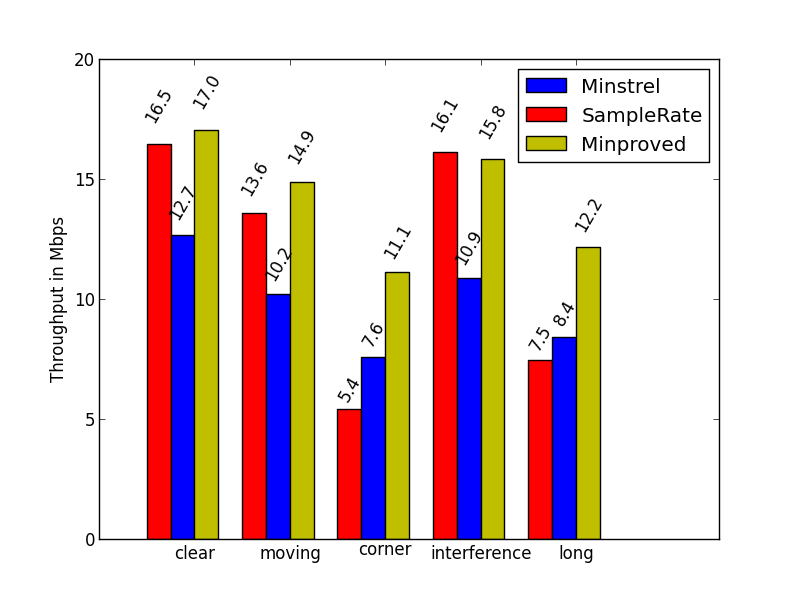
\includegraphics[width=\linewidth]{mnVSspVSmp1.png}
  \caption{Throughput of Minproved as compared to SampleRate and
    vanilla Minstrel.}
\label{figure:4}
\end{figure}

Overall, our improved Minstrel, which we call Minproved, often
out-performs Minstrel by multiple Mbps and never doing any worse; and
usually surpassing the best constant bit rate.  In only one case did
SampleRate achieve higher throughput than Minproved, and in this case
both surpassed the best constant bit-rate.  In cases where Minstrel
out-performed SampleRate, the same behavior was true of Minproved.  In
most cases, Minproved was $30\%$ faster than Minstrel, and in some the
improvement as great as $60\%$.

However, Minproved still makes many poor choices.  While a single
successful probe packet does not cause many hundreds of milliseconds
of failed packets, as it does in Minstrel, the single successful
packet can still cause one window's worth of failed packets.  Instead,
it would be best if a successful probe packet at a rarely-successful
bit-rate was treated more carefully.  One can imagine an algorithm,
for example, which would treat a single successful probe packet as a
reason to send a dozen more probe packets at that bit-rate, but does
not yet commit to sending hundreds of packets at that bit-rate.

However, these are only vague ideas, and we have no concrete
implementations of such an algorithm.


\section{Availability}

All of our code and collected trace data are available on GitHub:

\noindent
{\small\url{https://github.com/pavpanchekha/6.829-project/tree/3.8.6}}

This repository contains the modified \texttt{ath9k} driver used to
collect the traces, the traces we collected, as well as the Python
simulation framework.

\section{Future Work}

Very little analysis has been done of the performance of bit-rate
selection algorithms on 802.11n networks.  802.11n introduces many new
rates, as well as multiple-input/multiple output (MIMO) capabilities.
There is an 802.11n version of Minstrel, but there is no similar
implementation of SampleRate.

We implemented SampleRate as outlined in the thesis, but the MadWifi
implementation has a few key differences from the thesis.  MadWifi use
of an EWMA instead of a window has more accurate rate statistics,
which will potentially lead to better throughput.  We did not have the
time to implement this alternative version, but it is worth further
examination.

Hari Balakrishnan suggested that we use 802.11 broadcasts to collect
our traces, instead of link layer acknowledgments.  We would have
multiple computers listening at the broadcast address, and recording
all received packets.  If packets were sent over UDP, each computer's
record of which packets it received would allow us to compute the
success probability for each packet for each rate.  This approach
would free us from certain idiosyncrasies of reading data from the
driver, and lead to possibly more accurate traces, as well as the
ability to test multiple scenarios at once.  We were unable to
implement this due to a lack of time and inability to acquire
compatible hardware.

Finally, we are considering submitting our improvements to the
Minstrel algorithm, namely the balanced EWMA, as a kernel patch.
Currently our changes implemented in Python, so we would have to port
our improvements to C.

\section{Conclusion}

Minstrel and SampleRate perform similarly.  The results suggest that
SampleRate tends to perform slightly better, except in very lossy
links such as the client being far awat from the AP or actively
moving.  Minproved, our improved version of Minstrel, solidly
outperforms both Minstrel and SampleRate.

It seems that the replacement of SampleRate in the Linux kernel may
have been a hasty, since it seems to perform similarly to Minstrel and
it is a much simpler algorithm and thus simpler to adapt to changing
wireless standards.  We are not sure if adjustments to SampleRate can
bring its performance to match that of Minproved, however.

\section{Acknowledgments}

We would like to thank Jonathan Perry and Hari Balakrishnan for their
valuable guidance, as well as Derek Smithies for answering our
questions about Minstrel.

\bibliographystyle{acm}
\bibliography{paper}

\end{document}






